\documentclass[conference]{IEEEtran}
\usepackage{cite}
\usepackage{amsmath,amssymb,amsfonts}
\usepackage{algorithmic}
\usepackage{graphicx}
\usepackage{textcomp}
\usepackage{xcolor}
\usepackage{kotex}
\def\BibTeX{{\rm B\kern-.05em{\sc i\kern-.025em b}\kern-.08em
    T\kern-.1667em\lower.7ex\hbox{E}\kern-.125emX}}
\begin{document}

\title{Nanuda: A Group Expenses Manager}

\author{\IEEEauthorblockN{1\textsuperscript{st} Abia Herlianto}
\IEEEauthorblockA{\textit{School of Computer Science} \\
\textit{BINUS University}\\
\textit{Team MONEY}\\
Jakarta, Indonesia \\
abiaph@live.com}
\and
\IEEEauthorblockN{2\textsuperscript{nd} Hugo Ravé}
\IEEEauthorblockA{\textit{General Engineering} \\
\textit{ESILV PARIS-LA DEFENSE}\\
\textit{Team MONEY}\\
Paris, France \\
hugorave07@gmail.com}
\and
\IEEEauthorblockN{3\textsuperscript{rd} Nadya Hartanto}
\IEEEauthorblockA{\textit{School of Information Systems} \\
\textit{BINUS University}\\
\textit{Team MONEY}\\
Jakarta, Indonesia \\
ndhartanto1@gmail.com}
}

\maketitle

\begin{abstract}
Users create a "group" composed of either one person (themselves) or several people. Users then invite these people to the group. Users add expenses and split the costs with either all, some, or no members of the group. Users can add descriptions for each expense. Users can also customise how the costs are split. Users can see a summary of how much they owe to others and how much others owe to others. The summary of how much users owe changes as users spend and pay.
\end{abstract}

\begin{IEEEkeywords}
expenses, finance, management
\end{IEEEkeywords}

\begin{table}[htbp]
\caption{Role Assignments}
\label{tab:role-assignments}
\begin{tabular}{|c|c|c|}
\hline
\textbf{Role} & \textbf{Name} & \textbf{Task Description} \\ \hline
User/Customer &
  \begin{tabular}[c]{@{}c@{}}Nadya\\ Hartanto\end{tabular} &
  \begin{tabular}[c]{@{}c@{}}Tests the application for bugs and\\ issues. Provides feedback to the\\ Development Manager. Also provides\\ feedback on UX and UI quality.\end{tabular} \\ \hline
\begin{tabular}[c]{@{}c@{}}Software\\ Developer\end{tabular} &
  \begin{tabular}[c]{@{}c@{}}Abia Putrama\\ Herlianto\end{tabular} &
  \begin{tabular}[c]{@{}c@{}}Implements software based on design.\\ Fixes bugs and issues.\end{tabular} \\ \hline
\begin{tabular}[c]{@{}c@{}}Development\\ Manager\end{tabular} &
  Hugo Ravé &
  \begin{tabular}[c]{@{}c@{}}Designs software based on\\ requirements and feedback from\\ User/Customer. Organises,\\ schedules, and manages development.\end{tabular} \\ \hline
\end{tabular}
\end{table}

\section{Introduction}
When there are shared expenses in a group, it can be complicated to split the costs and gather the money that each person should pay. The usual solution is to have one or several individuals cover the cost of the entire group, and from there the remaining group members would pay their share to those who covered the cost.

The problem that arises from this is keeping track of these expenses. This is especially true for groups that meet regularly; for example, a group of friends going on a trip. Keeping track of who covered what for how much and who owes whom how much can quickly get out of hand. The solution that we propose is a simple application where these expenses can be organised, viewed, and accessed by all members of a certain group.

The name Nanuda comes from Korean 나누다, meaning 'to divide (up), to split (up)'. The name was chosen because our own experiences in splitting expenses in Korea was the reason we thought up of the idea.

There are several existing applications that perform a similar function, with different individual features. These include Tricount and Sesterce.
\begin{enumerate}
    \item \textbf{Tricount}
        \begin{figure}[htbp]
            \centerline{
\includegraphics[width=50mm,scale=0.5]{img/logo-tricount.png}}
            \caption{Tricount}
            \label{fig:tricount-logo}
        \end{figure}
        \\
        (Data from Google Play Store) \\
        Rating: 4.8 stars \\
        Downloads: 1 million+ \\
        Key features: Users can share a simple link to share their expenses. Members of a group can add expenses and see the balance. Expenses can be shared unevenly. Tricount works both offline and online, with logging in being optional. It also has both a mobile app and a website.
    \item \textbf{Sesterce}
        \begin{figure}[htbp]
            \centerline{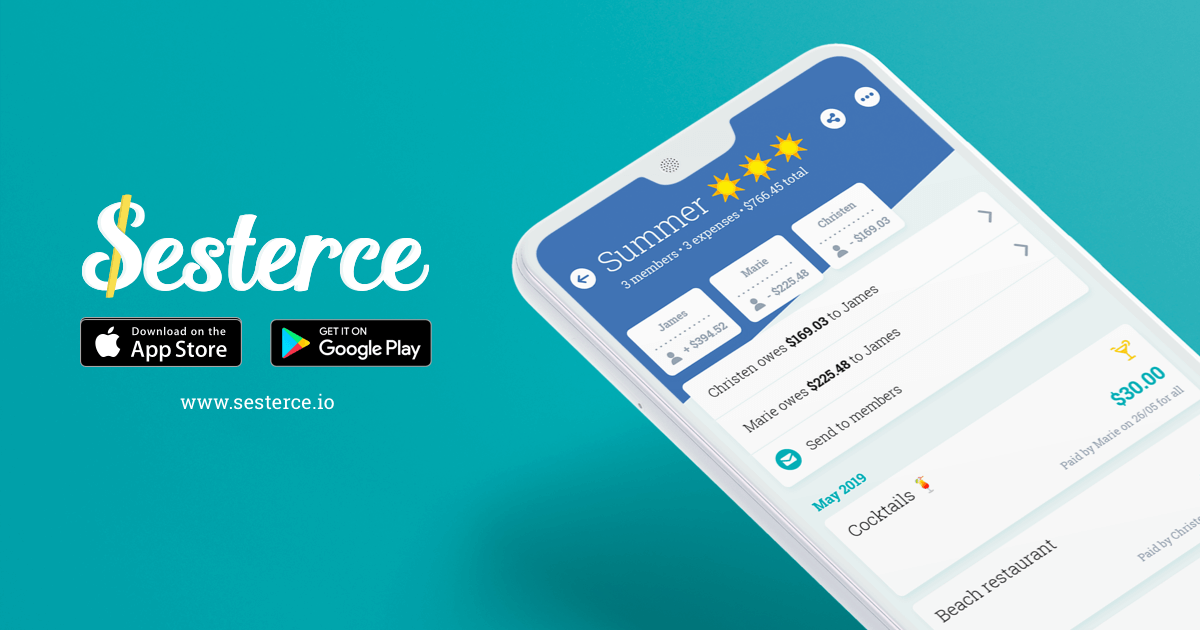
\includegraphics[width=50mm,scale=0.5]{img/logo-sesterce.png}}
            \caption{Sesterce}
            \label{fig:sesterce-logo}
        \end{figure}
        \\
        (Data from Google Play Store) \\
        Rating: 4.7 stars \\
        Downloads: 5,000+ \\
        Key features: Similar to Tricount, users can join a single group and add expenses, keeping track of all bills and costs. Sesterce is completely anonymous with no login or email required. In addition, Sesterce allows the addition of custom categories for expenses, the option to view statistics, and exporting all the data to a .csv file.
\end{enumerate}

\section{Requirements}

\begin{enumerate}
    \item This application should run on the Android operating system.
    \item This application should be able to run offline.
    \item \textbf{Loading Screen}
        \begin{enumerate}
            \item The application should load the locally stored groups data.
        \end{enumerate}
    \item \textbf{Groups}
        \begin{enumerate}
            \item The application should display existing, joined groups.
            \item The user should be able to open the groups.
            \item The user should be able to create new groups and join existing groups.
            \item The user should be able to join a group using a simple link.
            \item The user should be able to edit and delete existing, joined groups.
            \item The user should be able to save changes to and sync with the groups data in the server.
            \item By default, the application should display a sample group.
            \item A group should have one or more participants.
            \item A group should use only one currency out of several options.
        \end{enumerate}
    \item \textbf{Expenses}
        \begin{enumerate}
            \item The application should display existing expenses in the group.
            \item The user should be able to open the expenses.
            \item The user should be able to create new expenses in the group.
            \item The user should be able to edit and delete existing expenses.
            \item The user should be able to save changes to and sync with the group expenses data in the server.
            \item The user should be able to determine who pays and who owes.
            \item The user should be able to determine how much each participant owes.
        \end{enumerate}
    \item \textbf{Balances}
        \begin{enumerate}
            \item The application should display how much each participant currently owes or is owed in total.
            \item If a participant owes to another participant, the application should also show how much they owe only to that other participant.
        \end{enumerate}
\end{enumerate}

\section{Development Environment}
\subsection{Choice of Software Development Platform}
\begin{enumerate}
    \item \textbf{Platform}
        \newline
        \begin{figure}[htbp]
            \centerline{
\includegraphics[width=50mm,scale=0.5]{img/logo-android.png}}
            \caption{Android}
            \label{fig:android-logo}
        \end{figure}
        \newline
        For Nanuda, we have chosen the \textbf{Android} mobile operating system as the platform for several reasons:
        \begin{enumerate}
            \item Nanuda needs to be on a mobile platform for quick access and easy use
            \item Android is the best-selling mobile OS worldwide
            \item Resources for development on Android are widely available and at no cost
        \end{enumerate}
        
    \item \textbf{Programming Language}
        \newline
        \begin{figure}[htbp]
            \centerline{
\includegraphics[height=25mm,scale=0.5]{img/logo-java.png}}
            \caption{Java}
            \label{fig:java-logo}
        \end{figure}
        \newline
        For the development of Nanuda, we use the \textbf{Java} programming language. Java is a class-based, object-oriented programming language and one of the world's most popular and widely used programming languages. We chose to use Java for two reasons:
        \begin{enumerate}
            \item Java is the language used to develop Android apps through the Android SDK
            \item We are familiar with Java and have used it in the past
        \end{enumerate}
    \item \textbf{Cost Estimation}
        \newline
        For the development of Nanuda, all of the resources used are either free of charge or have both free and paid options. For the resources with free and paid options, we have decided to use the free option. As such, the development of Nanuda requires no cost.
        \begin{center}
            \begin{tabular}{|p{6em}|p{10em}|p{4em}|}
                \hline
                \textbf{Resource} & \textbf{Role Description} & \textbf{Cost} \\
                \hline
                Android Studio & Android Development IDE & 0 \\
                \hline
                AWS Educate & Backend Server & 0 \\
                \hline
                Overleaf & Online, Collaborative LaTeX Writing Tool & 0 \\
                \hline
                GitHub & Remote Repository and Version Control System & 0 \\
                \hline
                GitHub Desktop & GUI for GitHub & 0 \\
                \hline
            \end{tabular}
        \end{center}
    \item \textbf{Development Environment}
    \begin{itemize}
        \item \textbf{Android Studio Version 4.1} \\
        Android Studio was chosen because it is the official IDE for the Android operating system.
        \item \textbf{AWS Educate} \\
        AWS Educate is Amazon's programme for students to use AWS services at no cost.
        \item \textbf{Overleaf} \\
        Overleaf was chosen because of its popularity and the effectiveness of its features, namely simple, in-browser editing, immediate compilation, easy sharing and collaborative editing.
        \item \textbf{GitHub} \\
        GitHub was chosen for Nanuda's remote repository because of our familiarity with it in comparison to other version control systems.
        \item \textbf{GitHub for Desktop} \\
        GitHub for Desktop was chosen instead of the regular, CLI-based system to interact with GitHub because of its simplicity and intuitiveness.
    \end{itemize}
\end{enumerate}

\subsection{Software in use}
\begin{enumerate}
    \item \textbf{Tricount} \\
        \begin{figure}[htbp]
            \centerline{
\includegraphics[width=50mm,scale=0.5]{img/logo-tricount.png}}
            \caption{Tricount}
            \label{fig:my_label}
        \end{figure}
        \newline
        Starts by setting up your account, sign up/login through different ways (Facebook, phone number,etc...). Create your group by choosing a name, purpose of the group (trip, group of friends, couple, family) then choose your currency, add the name of the members (up to 30 participants) and finally share the link of the group to the members and you're all set to start keeping up with your expenses. 
        \newline
        Inside a group, you have two main pages: Expenses and Balance. Expenses is where you can see all the expenses of the group as well as the name of the group, who is in it, your total personal expenses and the total expenses of the group. An expense is presented on the screen like this: name of the expense, amount, currency, paid by who and date of the expense. You can click on it to see a picture of the object or receipt if it was added, modify the title of the expense, amount, date, paid by, and for who it was paid. You can also delete the expense. You can sort the expenses by different categories, such as amount paid, date of payment, payer and title.
        \newline
        The second main screen is Balance which shows who owes money and who is owed money. When you click on the owed money to someone, you can mark the debt as paid or you can invite them to pay you through a link sent via messaging platforms. 
        \newline
        You also have the main menu screen of the app which allows you to see all the groups you're a part of and where you can add or delete groups.
    \item\textbf{Sesterce} \\
        \begin{figure}[htbp]
            \centerline{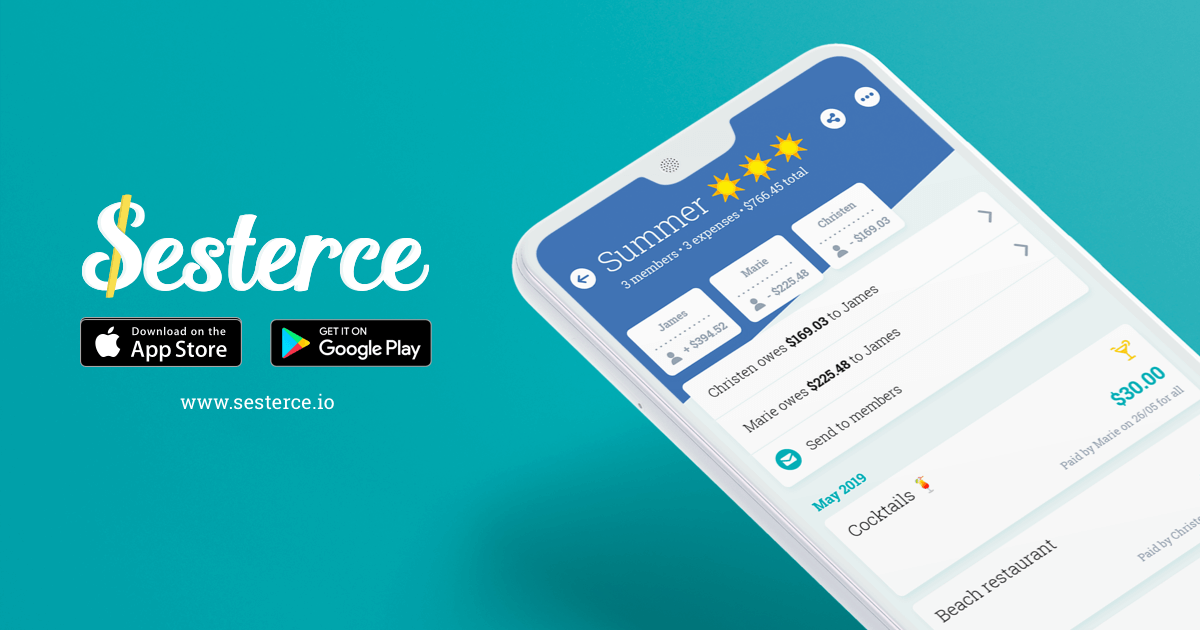
\includegraphics[width=50mm,scale=0.5]{img/logo-sesterce.png}}
            \caption{Sesterce}
            \label{fig:my_label}
        \end{figure}
        \newline
        The setup is pretty similar to create a group and add members.
        \newline
        There's only 1 main screen in Sesterce. It shows the group name, the number of members, the number of expenses, how much money was spent, who owes money or is owed money by whom. It also shows the list of all expenses sorted by date. The expenses display is pretty similar to Tricount as well, showing the title, the amount of the expense, who it is paid by and for whom. You can also add expenses. You have to chose who paid (one or multiple persons), the amount paid by each person, then select a title, add a date and choose a category for the expense (accommodation, groceries, transportation, you can even add your own category).  
\end{enumerate}

\section{Specifications}
    \begin{enumerate}
        \item \textbf{Loading Screen}
            \begin{enumerate}
                \item The application should load the locally stored groups data.
                \item If it is the first time the application is opened, the application should create new locally stored groups data. By default, a sample group with sample expenses should be made. After it is created, the new locally stored groups data should be uploaded to the server and added to the database.
            \end{enumerate}
        \item \textbf{Groups}
            \begin{enumerate}
                \item Groups List
                    \begin{enumerate}
                        \item The application should display a list of the existing locally stored groups.
                        \item For each group, its name and description are displayed.
                        \item Next to each group, there should be a delete button which if clicked should delete the group from the locally stored groups data.
                        \item The user should only be part of no more than 5 groups.
                    \end{enumerate}
                \item Enter Group
                    \begin{enumerate}
                        \item If the user clicks on a group, the application should move to the group's Expenses screen.
                    \end{enumerate}
                \item Add Group
                    \begin{enumerate}
                        \item If the user clicks the "Add Group" button, the application should display the "Add Group" pop up screen.
                        \item The application should display the "Make New Group" and "Join Group" buttons.
                        \item If the user is already part of 5 groups, the application should display an error informing the user that they have reached the maximum number of groups.
                    \end{enumerate}
                \item Make New Group
                    \begin{enumerate}
                        \item If the user clicks the "Make New Group" button, the application should display the "New Group" pop up screen.
                        \item The user should input the name of the new group, choose a currency to be used by the expenses in the group, and input the names of the participants of the new group.
                        \item The user should optionally be able to add a description to the new group.
                        \item The name of the new group should not be empty and should be no longer than 20 characters.
                        \item If there is a description, the description of the new group should be no longer than 50 characters.
                        \item The user should be able to choose one of at least three major currencies for the new group.
                        \item The user should be able to add participants' names by inputting the name and clicking the "Add" button.
                        \item The new group should have no more than 20 participants.
                        \item If the user clicks the "Create New Group" button, the application creates the new group and display a link to share to other users to join the group.
                        \item If the requirements for the new group have not been met, the "Create New Group" button should not be interactable.
                        \item If the user clicks the "Back" button, the application should move back to the groups list screen.
                    \end{enumerate}
                \item Join Group
                    \begin{enumerate}
                        \item If the user clicks the "Join Group" button, the application should display the "Join Group" pop up screen.
                        \item The user should input the link of the group they wish to join.
                        \item If the user clicks the "Join" button, the application sends a request to the server to find the group and download its information.
                        \item If the link has not been input or the link is invalid, the "Join" button should not be interactable.
                        \item If the user clicks the "Back" button, the application should move back to the groups list screen.
                    \end{enumerate}
                \item Sync Groups
                    \begin{enumerate}
                        \item If the user clicks the "Sync" button, the application should download the latest groups data from and upload changes to the server.
                    \end{enumerate}
            \end{enumerate}
        \item \textbf{Expenses}
            \begin{enumerate}
                \item Back Button
                    \begin{enumerate}
                        \item If the user clicks the "Back" button, the application should move back to the groups list screen.
                    \end{enumerate}
                \item Balances Button
                    \begin{enumerate}
                        \item If the user clicks the "Balances" button, the application should move to the balances screen.
                    \end{enumerate}
                \item Edit Group
                    \begin{enumerate}
                        \item If the user clicks the "Edit Group" button, the application should display the "Edit Group" pop up screen.
                        \item The application should display the name, currency used by, and names of the participants of the group.
                        \item The user should be able to change the name, the description, the currency used by the expenses in the group, and the names of the participants of the group.
                        \item The name of the group should not be empty and should be no longer than 20 characters.
                        \item If there is a description, the description of the group should be no longer than 50 characters.
                        \item The user should be able to choose one of at least three major currencies for the new group.
                        \item The user should be able to add participants' names by inputting the name and clicking the "Add" button.
                        \item The group should have no more than 20 participants.
                        \item If the user clicks the "Save Changes" button, the application updates the group and moves back to the expenses list screen.
                        \item If the requirements for the group have not been met, the "Save Changes" button should not be interactable.
                        \item If the user clicks the "Back" button, the application should move back to the expenses list screen.
                    \end{enumerate}
                \item Expenses List
                    \begin{enumerate}
                        \item The application should display a list of the existing locally stored expenses of the group.
                        \item For each expense, its name, amount, payer, and date should be displayed.
                        \item Next to each expense, there should be a delete button which if clicked should delete the expense from the locally stored data.
                        \item There should be no limit to the number of expenses in a group.
                    \end{enumerate}
                \item Enter Expense
                    \begin{enumerate}
                        \item If the user clicks on an expense, the application should display the details of the expense.
                        \item The application should display the name, amount, date, and payer of the expense. It should also display the participants who were paid for by this expense and how much each participant owes. It should also display the "Edit Expense" button.
                        \item If the user clicks the "Back" button, the application should move back to the expenses list screen.
                    \end{enumerate}
                \item Edit Expense
                    \begin{enumerate}
                        \item If the user clicks on the "Edit Expense" button, the application should display the "Edit Expense" pop up screen.
                        \item The application should display the name, amount, and date of the expense and choose the participant who pays and participants who are paid for.
                        \item The user should be able to change the name, amount, date of the expense, the participant who pays, and the participants who are paid for.
                        \item The name of the expense should not be empty and should be no longer than 20 characters.
                        \item The amount of the expense should not be empty.
                        \item The payer participant should not be empty and the user should choose a participant from the list of participants.
                        \item The application should display all the participants in the group under the "Paid For" label.
                        \item Next to each participant, there should be a checkbox so the user can choose whether the participant is paid for or not.
                        \item There should be a checkbox next to the "Paid For" label to choose all participants in the group.
                        \item Next to each participant whose checkbox is ticked, there should be the amount that will be owed by the participant. By default, the total amount expended should be divided equally between all paid for participants.
                        \item The user should optionally be able to change how much each participant will owe in the expense manually.
                        \item If the user edits how much each participant will owe in the expense manually, the total should be equal to the amount expended by the payer participant.
                        \item If the user clicks the "Save Changes" button, the application updates the expense and moves back to the expenses list screen.
                        \item If the requirements for the new expense have not been met, the "Save Changes" button should not be interactable.
                        \item If the user clicks the "Back" button, the application should move back to the expenses list screen.
                    \end{enumerate}
                \item Add Expense
                    \begin{enumerate}
                        \item If the user clicks the "Add Expense" button, the application should display the "New Expense" pop up screen.
                        \item The user should input the name, amount, and date of the expense and choose the participant who pays and the participants who are paid for.
                        \item The name of the expense should not be empty and should be no longer than 20 characters.
                        \item The amount of the expense should not be empty.
                        \item By default, the date of the expense should be the current date.
                        \item The payer participant should not be empty and the user should choose a participant from the list of participants.
                        \item The application should display all the participants in the group under the "Paid For" label.
                        \item Next to each participant, there should be a checkbox so the user can choose whether the participant is paid for or not.
                        \item There should be a checkbox next to the "Paid For" label to choose all participants in the group.
                        \item Next to each participant whose checkbox is ticked, there should be the amount that will be owed by the participant. By default, the total amount expended should be divided equally between all paid for participants.
                        \item The user should optionally be able to input how much each participant will owe in the expense manually.
                        \item If the user edits how much each participant will owe in the expense manually, the total should be equal to the amount expended by the payer participant.
                        \item If the user clicks the "Add Expense" button, the application creates the new expense and moves back to the expenses list screen.
                        \item If the requirements for the new expense have not been met, the "Add Expense" button should not be interactable.
                        \item If the user clicks the "Back" button, the application should move back to the expenses list screen.
                    \end{enumerate}
            \end{enumerate}
        \item \textbf{Balances}
            \begin{enumerate}
                \item Back Button
                    \begin{enumerate}
                        \item If the user clicks the "Back" button, the application should move back to the groups list screen.
                    \end{enumerate}
                \item Expenses Button
                    \begin{enumerate}
                        \item If the user clicks the "Expenses" button, the application should move to the expenses screen.
                    \end{enumerate}
                \item Summary
                    \begin{enumerate}
                        \item The application should display the name of each participant in the group and how much they owe or are owed to.
                        \item If in total the participant owes more than they are owed, then the total amount they owe should be displayed with a red background.
                        \item If in total the participant is owed more than they owe, then the total amount they are owed should be displayed with a green background.
                    \end{enumerate}
                \item Balancing Details
                    \begin{enumerate}
                        \item The application should display how much each participant owes another participant in separate balances. If A owes B and C, and B owes C, then the application should display how much A owes B, how much A owes C, and how much B owes C in separate balances.
                    \end{enumerate}
            \end{enumerate}
    \end{enumerate}
\end{document}
